\documentclass[tikz,border=6pt]{standalone}
\usepackage{amsmath,amssymb,mathtools,physics,bm,nicefrac,wasysym}
\usepackage{xcolor}

\definecolor{colone}{RGB}{180,60,60}
\definecolor{coltwo}{RGB}{60,110,180}
\definecolor{colthree}{RGB}{60,140,80}

\definecolor{accent}{HTML}{A13D2C}
\definecolor{accent2}{HTML}{2B5F6B}
\definecolor{muted}{HTML}{5A564F}
\definecolor{panel}{HTML}{F8F6F0}
\definecolor{linecol}{HTML}{D8D2C4}
\definecolor{ink}{HTML}{1E1C1A}
\definecolor{astroblue}{HTML}{1B4F72}
\definecolor{astrodark}{HTML}{17202A}
\definecolor{sunyellow}{HTML}{E8A33D}

\usetikzlibrary{calc,arrows.meta,positioning,decorations.pathreplacing,decorations.markings,angles,quotes,shapes.geometric}
\usepackage{tikz-3dplot}

\newcommand{\vecr}{\vec r}
\newcommand{\vecL}{\vec L}
\newcommand{\vecA}{\vec A}
\newcommand{\vecf}{\vec f}
\newcommand{\vecF}{\vec F}
\newcommand{\vecp}{\vec p}
\newcommand{\avg}[1]{\left\langle #1\right\rangle}
\newcommand{\vecx}{\vec x}
\newcommand{\hatn}{\hat n}
\newcommand{\rhat}{\hat r}
\newcommand{\phihat}{\hat\phi}
\newcommand{\thetahat}{\hat\theta}
\newcommand{\note}[1]{\textcolor{blue!60!black}{\textit{[#1]}}}

% Astronomical acronyms
\newcommand{\LST}{\mathrm{LST}}
\newcommand{\GST}{\mathrm{GST}}
\newcommand{\GMST}{\mathrm{GMST}}
\newcommand{\GAST}{\mathrm{GAST}}
\newcommand{\LMST}{\mathrm{LMST}}
\newcommand{\LAST}{\mathrm{LAST}}
\newcommand{\UT}{\mathrm{UT}}
\newcommand{\UTC}{\mathrm{UTC}}
\newcommand{\TAI}{\mathrm{TAI}}
\newcommand{\TT}{\mathrm{TT}}
\newcommand{\TDB}{\mathrm{TDB}}
\newcommand{\JD}{\mathrm{JD}}
\newcommand{\MJD}{\mathrm{MJD}}
\newcommand{\EoT}{\mathrm{EoT}}
\newcommand{\SNR}{\mathrm{SNR}}
\newcommand{\RON}{\mathrm{RON}}

% Helper commands for specific diagrams
\newcommand{\midlinelabel}[3]{
    \node (midlabel) at ($ (#1)!.5!(#2) $) {#3};
    \draw[stealth-] (#1) --  (midlabel);
    \draw[-stealth] (midlabel) -- (#2);
}
\newcommand{\midlinelabell}[3]{
    \node[fill = white, inner sep = 0.2pt, outer sep=3pt] (midlabel) at ($ (#1)!.5!(#2) $) {#3};
    \draw[stealth-] (#1) --  (midlabel);
    \draw[-stealth] (midlabel) -- (#2);
}
\newcommand{\midlinelabelll}[3]{
    \node[fill = white, inner sep = 0.2pt, outer sep=3pt,scale=0.6] (midlabel) at ($ (#1)!.5!(#2) $) {#3};
    \draw[stealth-] (#1) --  (midlabel);
    \draw[-stealth] (midlabel) -- (#2);
}



\usepackage[T1]{fontenc}\usepackage{newpxtext,newpxmath}  % same fonts as the notes
\begin{document}
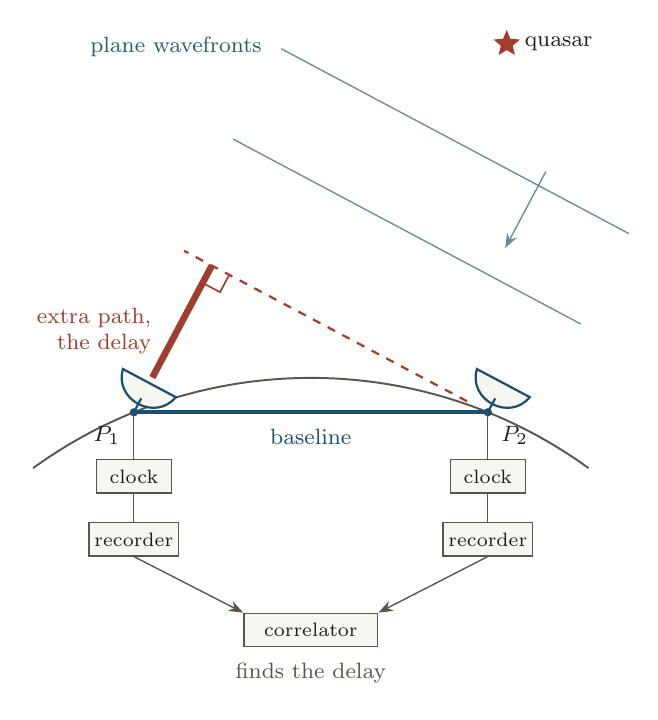
\begin{tikzpicture}[>=Stealth, lab/.style={font=\footnotesize, text=ink},
  box/.style={draw=muted, fill=panel, line width=0.5pt, font=\scriptsize, text=ink, inner sep=2pt, minimum height=0.42cm, minimum width=0.95cm}]
  \def\R{6}\def\ph{22}\def\a{28}
  \pgfmathsetmacro{\ux}{sin(\a)}   % direction towards the quasar is (ux,uy)
  \pgfmathsetmacro{\uy}{cos(\a)}
  \pgfmathsetmacro{\px}{\R*sin(\ph)}
  \pgfmathsetmacro{\py}{\R*cos(\ph)-\R}
  \coordinate (P1) at (-\px,\py);
  \coordinate (P2) at (\px,\py);
  \pgfmathsetmacro{\Lx}{2*\px*sin(\a)}   % extra path length
  \coordinate (W) at ($(P1)+(\Lx*\ux,\Lx*\uy)$);
  % Earth surface and chord
  \draw[muted, line width=0.7pt] ($(0,-\R)+({90-\ph-14}:\R)$) arc ({90-\ph-14}:{90+\ph+14}:\R);
  \draw[astroblue, line width=1.4pt] (P1) -- (P2);
  % wavefronts and quasar
  \foreach \s in {2.6,3.9}{
    \draw[accent2!70, line width=0.5pt] ($(0,\py)+(\s*\ux,\s*\uy)+(-2.5*\uy,2.5*\ux)$) -- ($(0,\py)+(\s*\ux,\s*\uy)+(2.5*\uy,-2.5*\ux)$);}
  \draw[accent2!70, line width=0.5pt, ->] ($(0,\py)+(3.9*\ux,3.9*\uy)+(1.2*\uy,-1.2*\ux)+(0.2*\ux,0.2*\uy)$) -- ++(-1.1*\ux,-1.1*\uy);
  \node[star, star points=5, star point ratio=2.2, fill=accent, draw=none, inner sep=1.6pt]
     (Q) at ($(0,\py)+(5.3*\ux,5.3*\uy)$) {};
  \node[lab, right=3pt] at (Q) {quasar};
  % wavefront through the second dish and the extra path to the first
  \draw[accent, dashed, line width=0.8pt] ($(P2)+(-0.3*\uy,0.3*\ux)$) -- ($(W)+(-0.4*\uy,0.4*\ux)$);
  \draw[accent, line width=2.4pt] (W) -- ($(P1)+(0.5*\ux,0.5*\uy)$);
  \draw[accent, line width=0.6pt] ($(W)+(0.25*\uy,-0.25*\ux)$) -- ++(-0.25*\ux,-0.25*\uy)  -- ++(-0.25*\uy,0.25*\ux);
  \node[lab, text=accent, anchor=east, align=right] at ($(W)!0.5!(P1)+(-0.15,0.1)$) {extra path,\\ the delay};
  % dishes
  \foreach \P in {P1,P2}{
    \begin{scope}[shift={(\P)}, rotate=-\a]
      \draw[astroblue, fill=panel, line width=0.8pt] (-0.38,0.42) .. controls (-0.3,0.02) and (0.3,0.02) .. (0.38,0.42) -- cycle;
      \draw[astroblue, line width=0.8pt] (0,0.2) -- (0,0);
    \end{scope}
    \fill[astroblue] (\P) circle (1.5pt);}
  \node[lab, below left=2pt] at (P1) {$P_1$};
  \node[lab, below right=2pt] at (P2) {$P_2$};
  % equipment inside the Earth
  \node[box] (c1) at (-\px,-1.25) {clock};
  \node[box] (r1) at (-\px,-2.05) {recorder};
  \node[box] (c2) at (\px,-1.25) {clock};
  \node[box] (r2) at (\px,-2.05) {recorder};
  \node[box, minimum width=1.7cm] (cor) at (0,-3.2) {correlator};
  \draw[muted, line width=0.4pt] (P1) -- (c1.north);
  \draw[muted, line width=0.4pt] (P2) -- (c2.north);
  \draw[muted, line width=0.4pt] (c1) -- (r1);
  \draw[muted, line width=0.4pt] (c2) -- (r2);
  \draw[->, muted, line width=0.5pt] (r1.south) -- (cor.north west);
  \draw[->, muted, line width=0.5pt] (r2.south) -- (cor.north east);
  \node[lab, text=astroblue] at (0,-0.75) {baseline};
  \node[lab, text=muted, anchor=north] at (0,-3.5) {finds the delay};
  \node[lab, text=accent2, anchor=east] at (-0.5,4.2) {plane wavefronts};
\end{tikzpicture}
\end{document}
